\subsection{Description}
The exponential distribution is the probability distribution of the time between events in a Poisson point process, i.e., a process in which events occur continuously and independently at a constant average rate. It is a particular case of the gamma distribution. It is the continuous analogue of the geometric distribution, and it has the key property of being memoryless. In addition to being used for the analysis of Poisson point processes it is found in various other contexts.


\subsubsection{Probability mass function}
\[
	f(x; \lambda) =
	\begin{cases}
		0 & \text{if } x < 0 \\
		\lambda e^{-\lambda x} & \text{if } x \geq 0
	\end{cases}
\]

\subsubsection{Cumulative distribution function}
\[
	F(x; \lambda) =
	\begin{cases}
		0 & \text{if } x < 0 \\
		1 - e^{-\lambda x} & \text{if } x \geq 0
	\end{cases}
\]

\subsubsection{Memorylessness}
See https://en.wikipedia.org/wiki/Exponential\_distribution


\subsection{Moments}

\begin{tabular}{p{0.5\textwidth} p{0.5\textwidth}}
	\hline
	Mean & $\frac{1}{\lambda}$ \\\hline
	Variance & $\frac{1}{\lambda ^2}$\\\hline
\end{tabular}

\subsection{Plots}


\begin{figure}[H]
	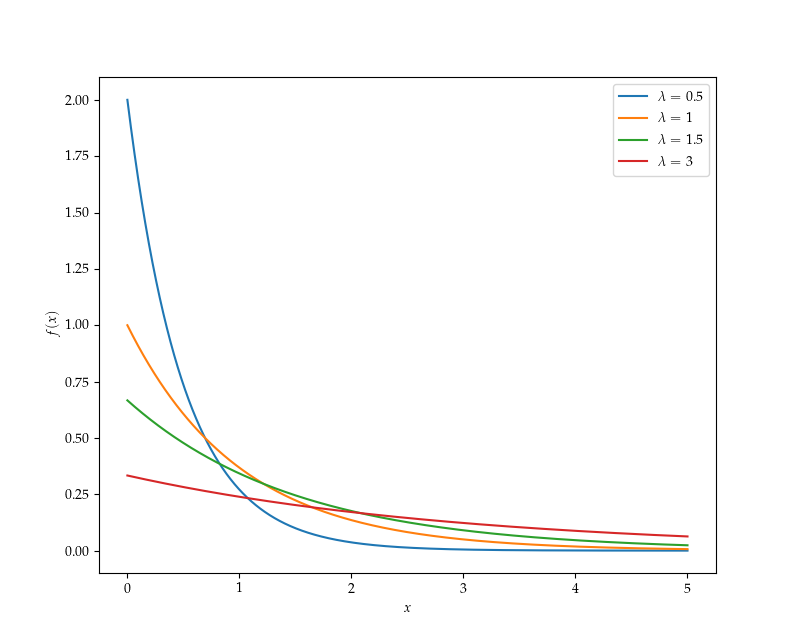
\includegraphics[width=\textwidth]{r/exponential/pdf.png}
\end{figure}
